\documentclass{exam}

\usepackage{amsmath,amssymb,amsfonts,amsthm,dsfont}
\usepackage{lib/extra}
\usepackage{graphicx}
\usepackage{tikz}
\usepackage{enumitem}
\usepackage{bbm}
\usepackage{pgfplots}
\usepackage{fontenc}
\usepackage{float}

\pgfplotsset{compat=1.18}
\renewcommand{\arraystretch}{1.5}
\setcounter{section}{2}

\title{Complex Analysis Chapter 1 Section 3}
\author{Brandyn Tucknott}
\date{Last Updated: 29 September 2025}

\begin{document}
\maketitle

\section{Integration along curves}
A \textbf{parameterized curve} $z(t)$ which maps a closed interval $[a, b] \subset \R$ to the complex plane. We say that the parameterized
curve is \textbf{smooth} if $z'(t)$ exists and is continuous on $[a, b]$ with $z'(t) \neq 0$ for $t\in [a ,b]$. At the points $t = a, b$,
$z'(a), z'(b)$ are interpreted as one-sided limits:
$$z'(a) = \lim_{h\to 0, h > 0} \frac{z(a + h) - z(a)}{h} \text{ and } z'(b) = \lim_{h\to 0, h < 0} \frac{z(b + h) - z(b)}{h}.$$
These quantities are called the right-handed derivative at $z(a)$ and left handed derivative at $z(b)$. We say the parameterized curve is
\textbf{piecewise-smooth} if $z$ is continuous on $[a, b]$ and there exist points $a = a_0 < a_1 < \hdots < a_n = b$,
where $z(t)$ is smooth on the intervals $[a_k, a_{k + 1}]$. The right-handed derivative and left-handed derivative at $a_k$ may differ for 
$k = 1, 2, \hdots, n - 1$.

Two parameterizations
$$z: [a, b]\to\C \text{ and } \tilde{z}: [c, d]\to \C$$
are \textbf{equivalent} if there exists a continuously differentiable bijection $s\to t(s)$ from $[c, d]\to[a, b]$ so that $t'(s) > 0$ and
$$\tilde{z}(s) = z(t(s)).$$

The condition $t'(s) > 0$ says that orientation must be preserved: as $s$ travels from $c$ to $d$, $t(s)$ travels from $a$ to $b$. The points
$z(a)$ and $z(b)$ are called \textbf{end-points} of the curve and are independent on the parameterization. Since a curve $\gamma$ carries an
orientation, it is natural to say that $\gamma$ begins at $z(a)$ and ends at $z(b)$. A smooth or piecewise-smooth curve is \textbf{closed}
if $z(a) = z(b)$ for any of its parameterizations, and \textbf{simple} if it is not self-intersecting ($z(t) \neq z(s)$ unless $s = t$).

\begin{figure}[H]
    \centering
    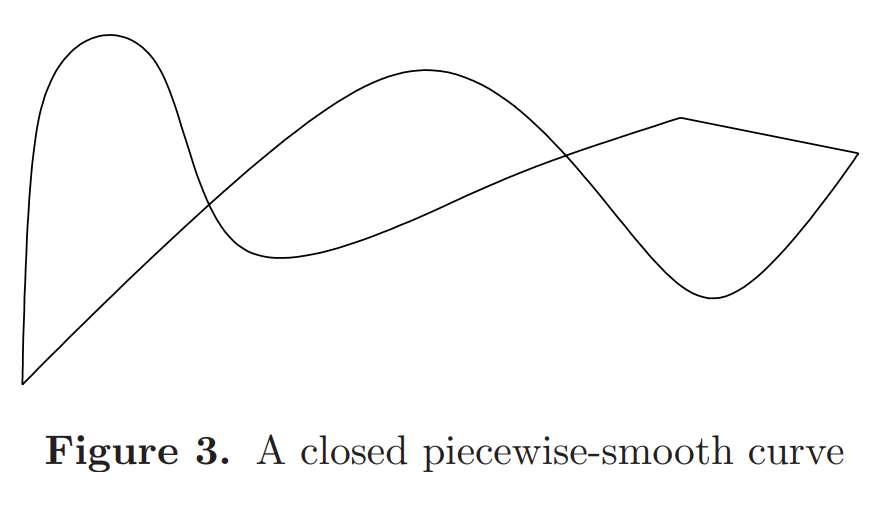
\includegraphics[width=0.5\textwidth]{figures/complex_analysis/figure_3.png}
\end{figure}

pg 39

\end{document}